%%%%%%%%%%%%%%%%%%%%%%%%%%%%%%%%%%%%%%%%%
% Vertical Line Title Page 
% LaTeX Template
% Version 1.0 (27/12/12)
%
% This template has been downloaded from:
% http://www.LaTeXTemplates.com
%
% Original author:
% Peter Wilson (herries.press@earthlink.net)
%
% License:
% CC BY-NC-SA 3.0 (http://creativecommons.org/licenses/by-nc-sa/3.0/)
% 
% Instructions for using this template:
% This title page compiles as is. If you wish to include this title page in 
% another document, you will need to copy everything before 
% \begin{document} into the preamble of your document. The title page is
% then included using \titleGM within your document.
%
%%%%%%%%%%%%%%%%%%%%%%%%%%%%%%%%%%%%%%%%%

%----------------------------------------------------------------------------------------
%	PACKAGES AND OTHER DOCUMENT CONFIGURATIONS
%----------------------------------------------------------------------------------------

\documentclass{report}

\usepackage{cite,graphicx}
\usepackage[chapter]{algorithm}
\usepackage{url,float}
\usepackage{hyperref}
\usepackage{uithesis}
\usepackage{listings}
\usepackage[nodayofweek,level]{datetime}
\usepackage[bahasai]{babel}
\selectlanguage{bahasai}
\renewcommand{\bibname}{Daftar Referensi}
\renewcommand{\contentsname}{Daftar Isi}
\renewcommand{\listfigurename}{Daftar Gambar}
\renewcommand{\listtablename}{Daftar Tabel}
\renewcommand\lstlistingname{Program}
\renewcommand\lstlistlistingname{Daftar Program}
%\def\lstlistingautorefname{Program.}
\renewcommand{\chaptername}{BAB}
\renewcommand{\figurename}{\bo{Gambar}}
\renewcommand{\tablename}{\bo{Tabel}}
\Var{\kataPengantar}{Kata Pengantar}
%
% Hyphenation untuk Indonesia 
%
% @author  Andreas Febrian
% @version 1.00
% 
% Tambahkan cara pemenggalan kata-kata yang salah dipenggal secara otomatis 
% oleh LaTeX. Jika kata tersebut dapat dipenggal dengan benar, maka tidak 
% perlu ditambahkan dalam berkas ini. Tanda pemenggalan kata menggunakan 
% tanda '-'; contoh:
% menarik
%   --> pemenggalan: me-na-rik
%

\hyphenation{
    % alphabhet A
    a-na-li-sa a-tur 
    a-pli-ka-si 
    % alphabhet B
    ba-ngun-an 
    be-be-ra-pa 
    ber-ge-rak
    ber-ke-lan-jut-an 
    ber-pe-nga-ruh 
    ber-o-pe-ra-si
    % alphabhet C
    ca-ri cri-ti-cal
    % alphabhet D
    di-sim-pan di-pim-pin de-ngan da-e-rah di-ba-ngun da-pat di-nya-ta-kan 
    di-sim-bol-kan di-pi-lih di-li-hat de-fi-ni-si
    di-mo-del-kan di-te-rap-kan
    di-ha-rap-kan
    di-e-va-lu-a-si
    di-su-sun
    di-sa-ji-kan
    % alphabhet E
    e-ner-gi eks-klu-sif
    % alphabhet F
    fa-si-li-tas
    % alphabhet G
    ga-bung-an ge-rak
    % alphabhet H
    ha-lang-an
    % alphabhet I
    % alphabhet J
    % alphabhet K
    ke-hi-lang-an
    ku-ning 
    kua-li-tas ka-me-ra ke-mung-kin-an ke-se-pa-ham-an
    % alphabhet L
    ling-kung-an
    % alphabhet M
    me-ne-ngah
    meng-a-tas-i me-mung-kin-kan me-nge-na-i me-ngi-rim-kan 
    meng-u-bah meng-a-dap-ta-si me-nya-ta-kan mo-di-fi-ka-si
    meng-a-tur
    meng-a-la-mi
    me-re-pre-sen-ta-si-kan
    men-da-pat-kan
    me-nun-juk-kan
    % alphabhet N
    nya-ta non-eks-klu-sif nu-klir
    % alphabhet O
    o-pe-ra-si
    % alphabhet P
	pe-nye-rap-an 
	pe-ngon-trol
    pe-mo-del-an
    pe-ran  pe-ran-an-nya
    pem-ba-ngun-an pre-si-den pe-me-rin-tah prio-ri-tas peng-am-bil-an 
    peng-ga-bung-an pe-nga-was-an pe-ngem-bang-an 
    pe-nga-ruh pa-ra-lel-is-me per-hi-tung-an per-ma-sa-lah-an 
    pen-ca-ri-an peng-struk-tur-an
    per-siap-an pa-ra-me-ter
    pa-sang-an
    % alphabhet Q
    % alphabhet R
    ran-cang-an
    % alphabhet S
    si-mu-la-si sa-ngat
    % alphabhet T
    te-ngah
    ter-da-pat
    % alphabhet U
    % alphabhet V
    % alphabhet W
    % alphabhet X
    % alphabhet Y
    % alphabhet Z
    % special
}


%----------------------------------------------------------------------------------------
%	TITLE PAGE
%----------------------------------------------------------------------------------------

\newcommand*{\titleGM}{\begingroup % Create the command for including the title page in the document
\hbox{ % Horizontal box
\hspace*{0.2\textwidth} % Whitespace to the left of the title page
\rule{1pt}{\textheight} % Vertical line
\hspace*{0.05\textwidth} % Whitespace between the vertical line and title page text
\parbox[b]{0.75\textwidth}{ % Paragraph box which restricts text to less than the width of the page

{\noindent\Huge\bfseries Pemrograman Python untuk Pengolahan Citra Digital }\\[2\baselineskip] % Title
{\large \textit{Diktat kuliah}}\\[4\baselineskip] % Tagline or further description
{\large \textsc{Dr. Arya Adhyaksa Waskita}} % Author name

\vspace{0.5\textheight} % Whitespace between the title block and the publisher
\begin{figure}[H]

\includegraphics[scale=.2]{pics/logo.png}
\end{figure}
STMIK Eresha - 2020
%Powered by \LaTex

%{\noindent The Publisher \plogo}\\[\baselineskip] % Publisher and logo
}}
\endgroup}

%----------------------------------------------------------------------------------------
%	BLANK DOCUMENT
%----------------------------------------------------------------------------------------

\begin{document}

%\addChapter{\kataPengantar}


\pagestyle{empty} % Removes page numbers

\titleGM % This command includes the title page
\pagenumbering{roman}
\setcounter{page}{0}
\tableofcontents
\listoffigures
\addChapter{Daftar Program}
\lstlistoflistings
\addChapter{\kataPengantar}
%-----------------------------------------------------------------------------%
\chapter*{Kata Pengantar}
%-----------------------------------------------------------------------------%
Diktat kuliah ini hanya merupakan pelengkap agar mahasiswa dapat lebih mudah memahami materi pengolahan citra digital. Penggunaan ilustrasi lain dari perangkat lunak berbayar dapat saja diberikan. Tetapi, karena pertimbangan kemandirian dan lisensi, maka saya memutuskan untuk menyusun diktat ini berbasis pada pustaka berlisensi publik dan berbasis bahasa pemrograman Python, \texttt{scikit-image}. Python dipertimbangkan karena banyak pustaka ilmiah yang sudah umum digunakan dan terus dikembangkan yang berbasis pada Python. Dalam pengolahan citra, selain \texttt{scikit-image}, ada juga \texttt{OpenCV} untuk \textit{Computer Vision}. Dalam pembelajaran mesin, \texttt{scikit-learn} adalah pustaka yang juga banyak digunakan. Bahkan \texttt{tensorflow}, pustaka yang banyak digunakan dalam penelitian \textit{deep learning} juga berbasis pada Python. Saya yakin, dengan mempelajari diktat ini, mahasiswa mampu mandiri dalam penguasaan bahasa pemrograman Python yang pada akhirnya mampu membuat mahasiwa lebih adaptif terhadap pustaka berbasis python, baik untuk tujuan ilmiah maupun bisnis. Mahasiswapun diharapkan menjadi lebih kreatif dalam melakukan penelitian hingga mengembangkan produk perangkat lunak, maupun prototipe perangkat keras cerdas berbasis Python tanpa harus terbebani masalah lisensi.

Secara umum, diktat ini dibagi ke dalam bagian pendahuluan yang membahas tentang sejarah singkat Python yang dilanjutkan ke bagian instalasi. Instalasi ini, meskipun sangat sederhana, terutama pada sistem operasi Linux, dapat menjadi sangat merepotkan bagi beberapa mahasiswa, terutama ketika mereka menggunakan sistem operasi Windows. Karena itu, instalasi akan dilakukan di sistem operasi Windows. Bagian selanjutnya adalah dasar-dasar pemrograman Python, terutama struktur data (\texttt{list}, \texttt{tuple} dan \texttt{dictionary}), interaksi dengan \textit{file}, hingga mempelajari penggunaan fungsi yang terdapat dalam pustaka tertentu. Sedangkan bagian terkahir dari diktat ini akan sepenuhnya diisi dengan fitur pustaka \texttt{scikit-image}, yang saat diktat ini disusun berada pada rilis \texttt{0.17.2}.
\clearpage
Diktat ini tidak ditujukan untuk menjadi rujukan dalam teknik pengolahan citra. Sehingga penjelasan teoritis terkait pengolahan citra akan diberikan dalam porsi yang sangat minim dan hanya ditujukan sebegai pelengkap saja. Selain itu, dalam diktat ini banyak menggunakan sumber dari situs web dan akan disampaikan secara detil alamat sumber tersebut dalam diktat. Diharapkan, mahasiswa tidak takut mencoba karena ada begitu banyak sumber yang dapat digunakan untuk belajar. Hanya kesungguhan kitalah yang akan menjadi pembeda. Akhirnya, selamat mencoba pengalaman baru. 

\vspace*{2cm}
\begin{flushright}
\selectlanguage{bahasai}
Serpong, \today\\[0.1cm]
\vspace*{1cm}
Dr. Arya Adhyaksa Waskita

\end{flushright}


\pagenumbering{arabic}
\chapter{Sejarah Pemrograman Python}

\chapter{Instalasi Python}
\section{Sejarah singkat}
Python dibangun oleh Guido van Rossum (\figurename~\ref{fig:guido}\footnote{\url{https://gvanrossum.github.io/images/guido-headshot-2019.jpg}}) pada sekitar tahun 1980 di \textit{Centrum Wiskunde \& Informatica} (CWI) di Belanda\cite{python3intro}. Nama Python diambil dari program TV favorit Guido yang berjudul '''Monty Pythons Flying Circus''' yang tayang pada kisaran tahun 1969-1974.

\begin{figure}
  \begin{center}
    \includegraphics[scale=.5]{pics/guido-headshot-2019.jpg}
    \caption{Guido van Rossum}
    \label{fig:guido}
  \end{center}
\end{figure}

\section{Interpreter Python}
\label{sec:interpreter}
Seperti telah dijelaskan di bagian Pengantar, instalasi \textit{interpreter} Python dilakukan di sistem operasi Windows 7. Tahapan instalasi ini mengasumsikan bahwa tidak ada kendala apapun terkait sistem operasi. Selanjutnya mahasiwa diminta untuk mengunduh \textit{interpreter} Python melalui laman \url{https://www.python.org/downloads/} sesuai kebutuhannya. 

Mengeksekusi unduhan tersebut akan memunculkan dialog seperti pada \figurename~\ref{fig:install1}. Pastikan untuk memilih konfigurasi \texttt{PATH} secara otomatis agar ketika proses instalasi selesai, \textit{interpreter} Python dapat dijalankan dari mana saja di sistem komputer masing-masing. Untuk kondisi di mana terjadi kesalahan, akan muncul dialog yang memberi kita kesempatan untuk melihat \textit{log}. Buka log tersebut dan lihat sumber dari kesalahan instalasi yang sedang terjadi.

\begin{figure}[h!]
   \begin{center}
     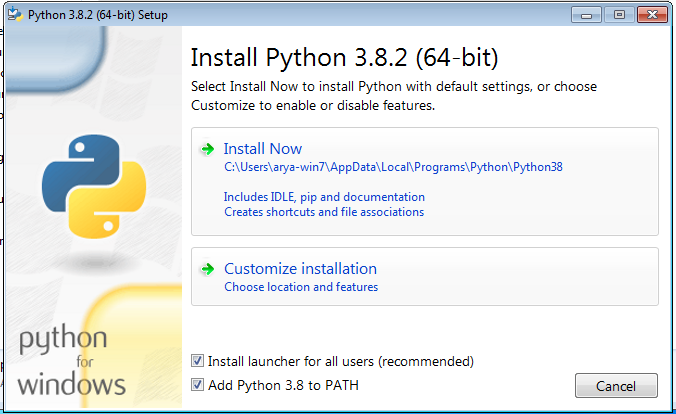
\includegraphics[scale=.5]{pics/installPython1.png}
     \caption{Dialog instalasi \textit{interpreter} Python}
     \label{fig:install1}
   \end{center}
 \end{figure} 

Pilihan opsi \textit{Customize installation} akan menampilkan dialog seperti \figurename~\ref{fig:feature}. Pastikan semua pilihan dipilih. Kemudian, selama proses instalasi berlangsung, pengguna akan disuguhkan dialog seperti \figurename~\ref{fig:installProgres}. Tunggu sampai dialog tanda selesai dikeluarkan seperti pada \figurename~\ref{fig:finish}.

\begin{figure}[h!]
  \begin{center}
    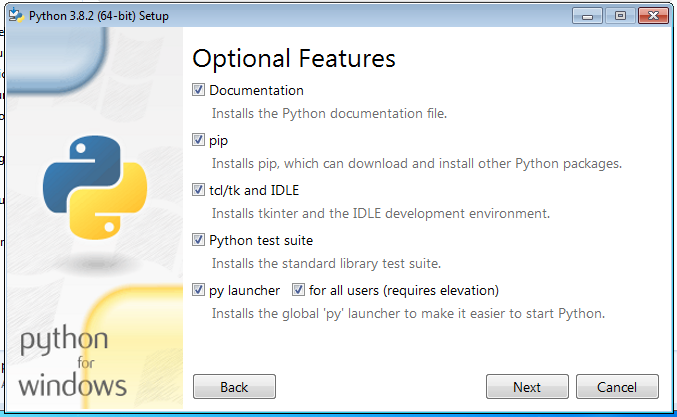
\includegraphics[scale=.5]{pics/featureInstall.png}
    \caption{Pilihan paket pendukung sebelum instalasi dilakukan}
    \label{fig:feature}
  \end{center}
\end{figure}

\begin{figure}[h!]
  \begin{center}
    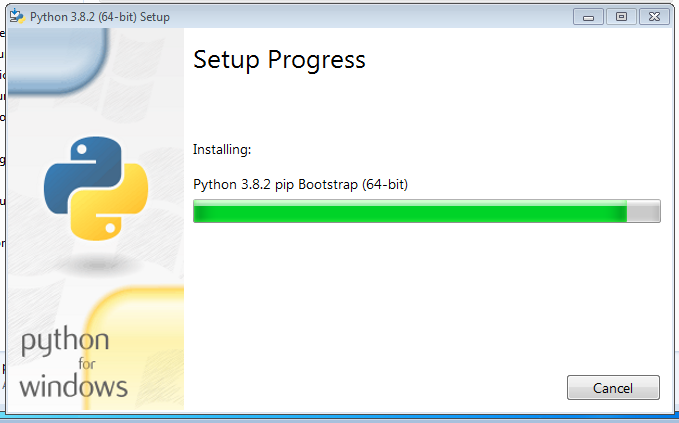
\includegraphics[scale=.5]{pics/installProgress.png}
    \caption{Dialos selama proses instalasi berlangsung}
    \label{fig:installProgres}
  \end{center}
\end{figure}

\begin{figure}[h!]
  \begin{center}
    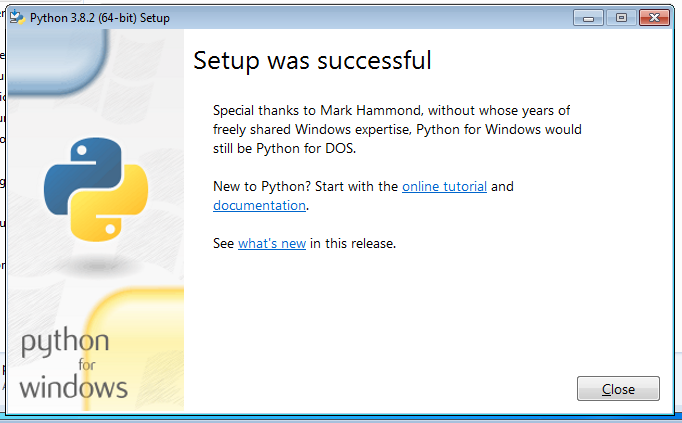
\includegraphics[scale=.5]{pics/installFinished.png}
    \caption{Dialog tanda selesai instalasi}
    \label{fig:finish}
  \end{center}
\end{figure}

Seperti telah ditunjukkan pada \figurename~\ref{fig:install1} tentang informasi lokasi \textit{interpreter} Python diletakkan, dapat juga dibuktikan melalui aplikasi \texttt{CMD} seperti \figurename~\ref{fig:lokasi}. Sedangkan \textit{interpreter} Python dapat diujicobakan dengan menuliskan perintah \texttt{python} di aplikasi \texttt{CMD}. Akan muncul dialog seperti \figurename~\ref{fig:siap}. \textit{Interpreter} Python siap digunakan, ditandai dengan munculnya karakter \texttt{>>>}.

\begin{figure}[h!]
  \begin{center}
    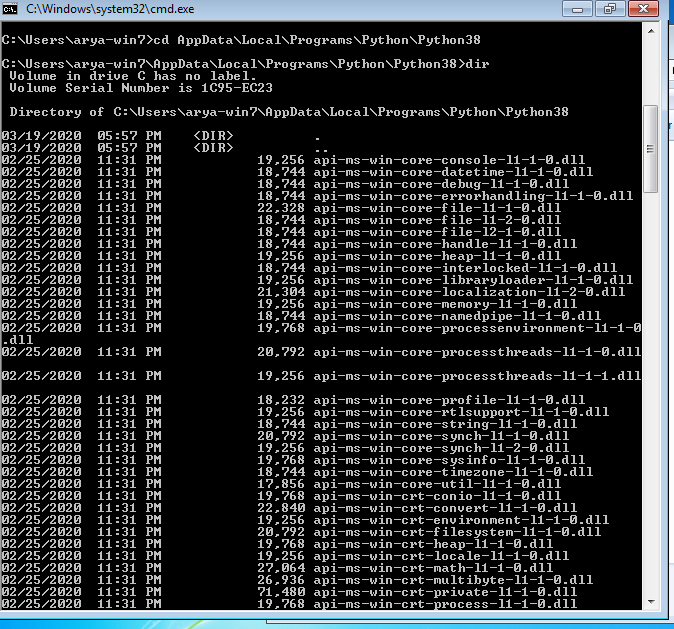
\includegraphics[scale=.5]{pics/installedLocation.png}
    \caption{Lokasi instalasi \textit{interpreter} Python}
    \label{fig:lokasi}
  \end{center}
\end{figure}

\begin{figure}[h!]
  \begin{center}
    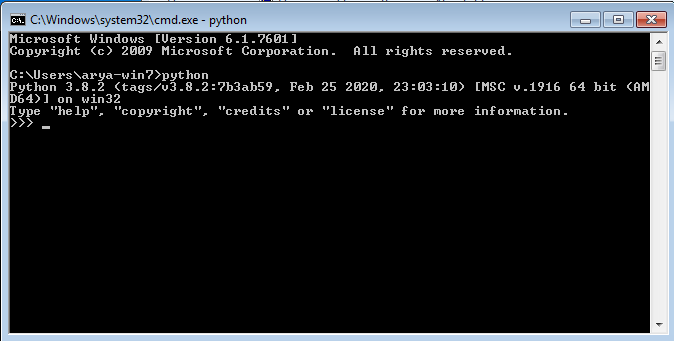
\includegraphics[scale=.5]{pics/pythonAktif.png}
    \caption{\textit{Interpreter} Python siap digunakan}
    \label{fig:siap}
  \end{center}
\end{figure}

Tahapan selanjutnya adalah instalasi pustaka \texttt{scikit-image}. Proses instalasinya dilakukan dengan aplikasi pengelola paket Python yang bernama \texttt{pip}. Silakan lihat \figurename~\ref{fig:feature}. \texttt{pip} ada di urutan kedua dari fitur tambahan. \texttt{pip} dapat digunakan untuk melihat paket apa saja yang telah terpasang di sistem kita. Caranya dengan menjalankan perintah \texttt{python -m pip list} seperti ditunjukkan \figurename~\ref{fig:daftarPaket}.

\begin{figure}[h!]
  \begin{center}
    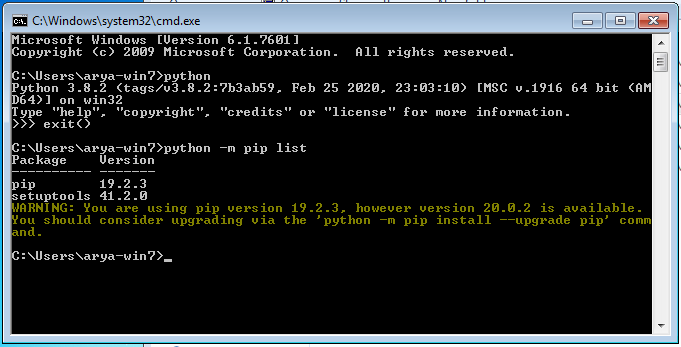
\includegraphics[scale=.5]{pics/pipList.png}
    \caption{Daftar paket yang terpasang}
    \label{fig:daftarPaket}
  \end{center}
\end{figure}

\texttt{pip} dapat juga digunakan untuk meng-\texttt{upgrade} paket yang telah terpasang, bahkan dirinya sendiri. Untuk meng-\textit{upgrade} paket \texttt{pip} itu sendiri, dapat dilakukan dengan menjalankan perintah \texttt{python -m pip install --upgrade pip} seperti \figurename~\ref{fig:pipUpgrade}. Perhatikan versi \texttt{pip} yang ada di \figurename~\ref{fig:daftarPaket} dan \figurename~\ref{fig:pipUpgrade}.
 
\begin{figure}
  \begin{center}
    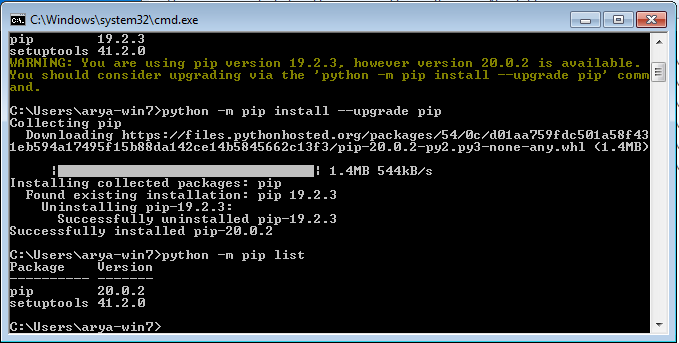
\includegraphics[scale=.5]{pics/pipList2.png}
    \caption{Hasil \texttt{upgrade} pip}
    \label{fig:pipUpgrade}
  \end{center}
\end{figure}

Sedangkan untuk memasang pustaka \texttt{scikit-image}, jalankan perintah \texttt{python -m pip install scikit-image} pada aplikasi \texttt{CMD} seperti \figurename~\ref{fig:installSkimage}.

\begin{figure}[h!]
  \begin{center}
    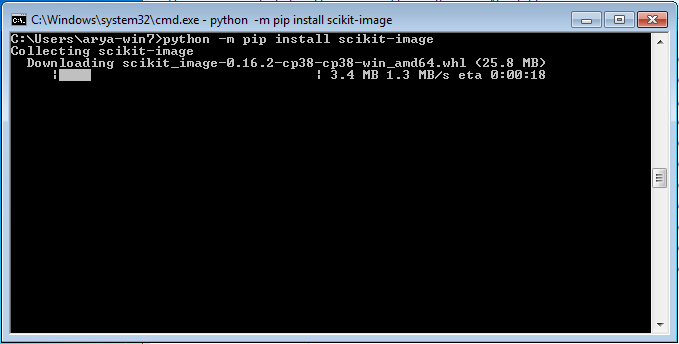
\includegraphics[scale=.5]{pics/installScikit-Image.png}
    \caption{Instalasi pustaka \texttt{scikit-image} menggunakan \texttt{pip}}
    \label{fig:installSkimage}
  \end{center}
\end{figure}

Jika ada pustaka lain yang menjadi ketergantungan dari pustaka yang akan diinstal, pip akan melakukan instalasi secara otomatis. \figurename~\ref{fig:installDepend} menunjukkan proses tersebut. Hal ini akan sangat memudahkan pengguna mengelola pustaka Python yang digunakan.

\begin{figure}[h!]
  \begin{center}
    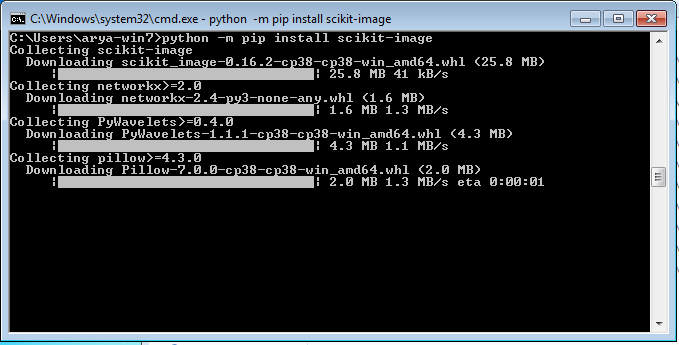
\includegraphics[scale=.5]{pics/installScikit-Imagedependencies.png}
    \caption{Instalasi pustaka \textit{dependent}}
    \label{fig:installDepend}
  \end{center}
\end{figure}

Setelah selesai, kita dapat kembali melihat daftar paket yang terpasang melalui pengelolaan \texttt{pip} yang ditunjukkan \figurename~\ref{fig:daftarPaket2}.

\begin{figure}[h!]
  \begin{center}
    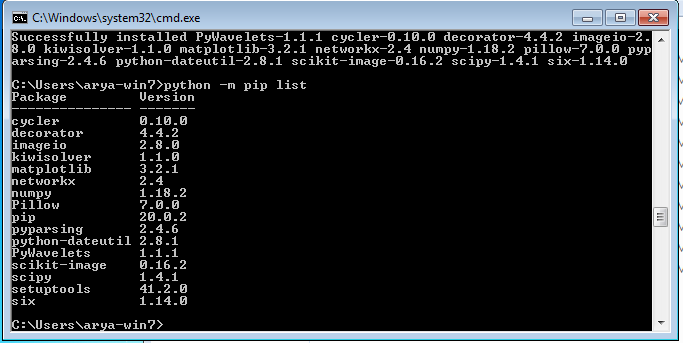
\includegraphics[scale=.5]{pics/pipList3.png}
    \caption{Daftar terakhir paket terpasang}
    \label{fig:daftarPaket2}
  \end{center}
\end{figure}

Menu aplikasi pendukung Python akan muncul seperti \figurename~\ref{fig:menu}. Menu kedua pada \figurename~\ref{fig:menu} akan memunculkan aplikasi \texttt{CMD} yang sama dengan yang ditunjukkan \figurename~\ref{fig:siap}, tetapi tanpa perlu memanggil perintah \texttt{python} terlebih dahulu. CMD secara otomatis akan memunculkan Python \texttt{shell} seperti \figurename~\ref{fig:siap}.

\begin{figure}[h!]
  \begin{center}
    \includegraphics[scale=.5]{pics/menuPython.png}
    \caption{Daftar menu aplikasi pendukung Python}
    \label{fig:menu}
  \end{center}
\end{figure}

\texttt{IDLE} adalah antarmukan \textit{interpreter} Python seperti ditunjukkan \figurename~\ref{fig:idle}. Dalam \figurename~\ref{fig:idle} juga terlihat bahwa kita berhasil meng-\textit{import} pustaka \texttt{scikit-image}, yang dalam \texttt{IDLE} di Windows 7 disebut sebagai \texttt{skimage}. Jika Anda sedang menggunakan Ubuntu, kemudian menggunakan pustaka \texttt{scikit-image} yang diperoleh dari \textit{repository} Ubuntu (bukan dari \texttt{pip}), pustaka \texttt{scikit-image} juga di-\textit{import} dengan nama \texttt{skimage}. Berhasilnya sebuah pustaka Python di-\textit{import} adalah ketika tidak ada komentar yang muncul setelah perintah \texttt{import} tersebut.

\begin{figure}
  \begin{center}
    \includegraphics[scale=.5]{pics/idle.png}
    \caption{Aplikasi \texttt{IDLE}}
    \label{fig:idle}
  \end{center}
\end{figure}

Selanjutnya, jika ditemukan petunjuk untuk masuk ke Python \texttt{Shell}, Anda dapat menggunakan aplikasi \texttt{IDLE}\texttt{}, atau menggunakan terminal (di Linux)/\texttt{CMD} (di Windows) dengan terlebih dahulu menjalankan perintah \texttt{python}.

\section{Anaconda}
Selain pilihan manual seperti yang telah dijelaskan di Sub bab \ref{sec:interpreter}, Anaconda bisa menjadi opsi lain yang lebih bersifat otomatis. Saya menyebutnya otomatis karena Anaconda sejumlah pustaka Python, terutama yang banyak digunakan di \textit{Data Mining}, \textit{Machine Learning} atau \textit{Data Science} telah dikemas di dalam Anaconda. Bahkan beberapa editor yang populer untuk Python juga dikemasnya. Anaconda bahkan mengemasnya khusus untuk \textit{platform} yang berbeda. Anda dapat menghubungi alamat \url{https://www.anaconda.com/} untuk mengunduh aplikasinya. Sesuaikan kebutuhan Anda dengan pilihan yang ada seperti ditunjukkan \figurename~\ref{fig:platformAnaconda}.

\begin{figure}[h!]
  \begin{center}
    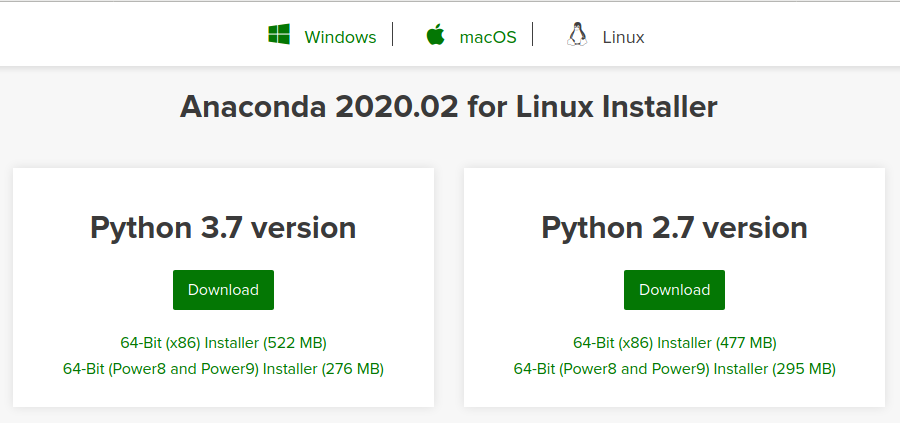
\includegraphics[scale=.5]{pics/anacondaInstall0.png}
    \caption{Pilihan \textit{platform} instalasi Anaconda}
    \label{fig:platformAnaconda}
  \end{center}
\end{figure}

Instalasi Anaconda akan menghadirkan dialog seperti ditunjukkan \figurename~\ref{fig:pembuka} - \figurename~\ref{fig:instalasiEnd}. Anaconda akan meletakkan pustaka di lokasi \texttt{C:\textbackslash\textbackslash ProgramData\textbackslash\textbackslash Anaconda3} yang berbeda dengan \texttt{pip} seperti terlihat di \figurename~\ref{fig:target}. Sedangkan di \figurename~\ref{fig:prosesInstalasi} terlihat sejumlah pustaka penting seperti \texttt{scikit-image} dan \texttt{scikit-learn} tengah diinstal. 

\begin{figure}aplikasi ini akan menghadirkan antarmuka seperti tampak
  \begin{center}
    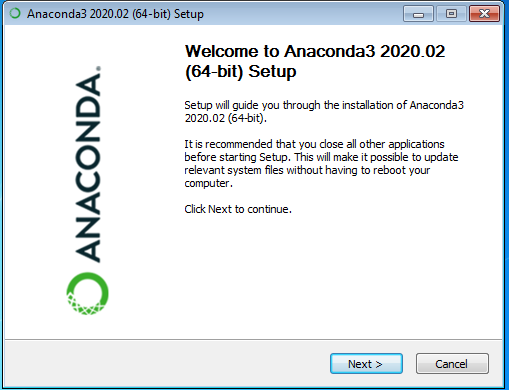
\includegraphics[scale=.5]{pics/anacondaInstall1.png}
    \caption{Dialog pembuka instalasi}
    \label{fig:pembuka}
  \end{center}
\end{figure}

\begin{figure}[h!]
  \begin{center}
    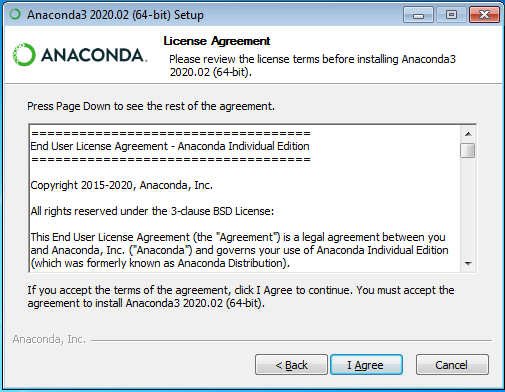
\includegraphics[scale=.5]{pics/anacondaInstall2.png}
    \caption{Menyetujui kesepakatan}
    \label{fig:kesepakatan}
  \end{center}
\end{figure}

\begin{figure}[h!]
  \begin{center}
    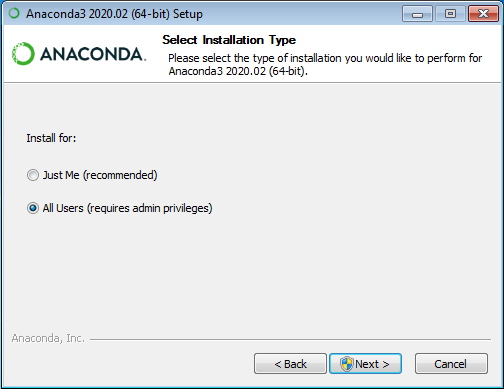
\includegraphics[scale=.5]{pics/anacondaInstall3.png}
    \caption{Pilihan pengguna Anaconda}
    \label{fig:pengguna}
  \end{center}
\end{figure}

\begin{figure}[h!]
  \begin{center}
    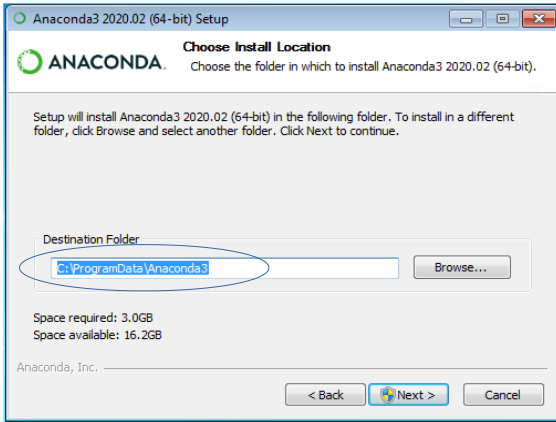
\includegraphics[scale=.5]{pics/anacondaInstall4a.png}
    \caption{Target instalasi}
    \label{fig:target}
  \end{center}
\end{figure}

\begin{figure}[h!]
  \begin{center}
    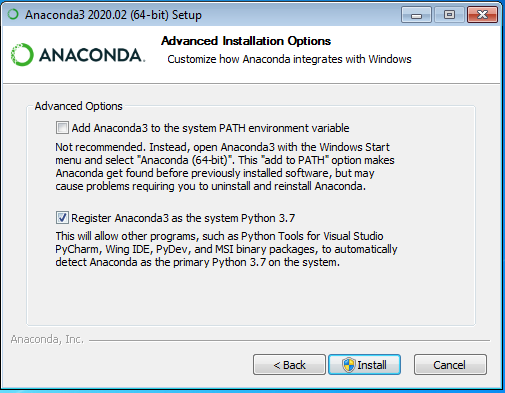
\includegraphics[scale=.5]{pics/anacondaInstall5.png}
    \caption{Menjadikan Anaconda sebagai sistem utama Python}
    \label{fig:utama}
  \end{center}
\end{figure}

\begin{figure}[h!]
  \begin{center}
    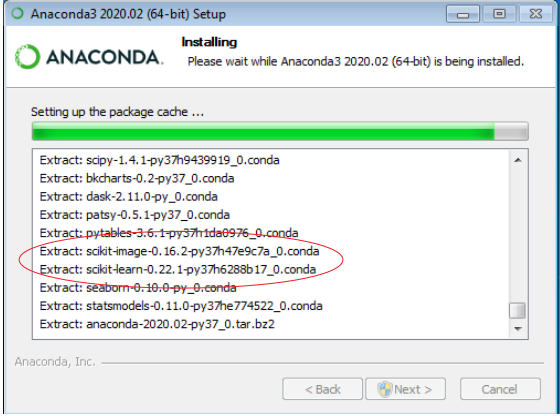
\includegraphics[scale=.5]{pics/anacondaInstall6a.png}
    \caption{Proses instalasi}
    \label{fig:prosesInstalasi}
  \end{center}
\end{figure}

\begin{figure}[h!]
  \begin{center}
    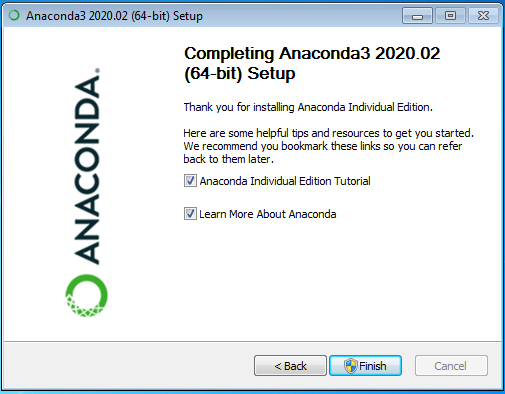
\includegraphics[scale=.5]{pics/anacondaInstall9.png}
    \caption{Instalasi selesai}
    \label{fig:instalasiEnd}
  \end{center}
\end{figure}

Instalasi Anaconda akan membuat menu seperti pada \figurename~\ref{fig:menuAnaconda}. Di situ terlihat sejumlah aplikasi yang dapat digunakan untuk mengembangkan kode komputer berbasis Python seperti Jupyter dan Spyder. Untuk Jupyter, aplikasi ini akan menghadirkan antarmuka seperti tampak pada \figurename~\ref{fig:jupyter}. Di sisi kanan atas terlihat beberapa opsi antarmuka untuk mengelola proyek Python dengan Jupyter, seperti Terminal \figurename~\ref{fig:jupyterTerminal} atau Python \texttt{Shell} di bawah Jupyter seperti \figurename~\ref{fig:jupyterShell} yang perannya seperti \texttt{IDLE} di \figurename~\ref{fig:idle}. Sedangkan untuk Spyder, akan tampak antarmuka seperti \figurename~\ref{fig:spyder}.

\begin{figure}[h!]
  \begin{center}
    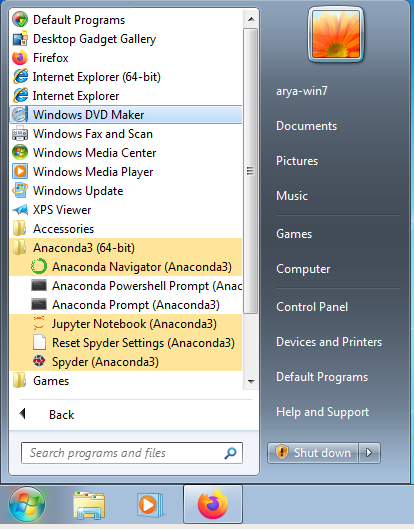
\includegraphics[scale=.5]{pics/anacondaMenu2.png}
    \caption{}
    \label{fig:menuAnaconda}
  \end{center}
\end{figure}

\begin{figure}
  \begin{center}
    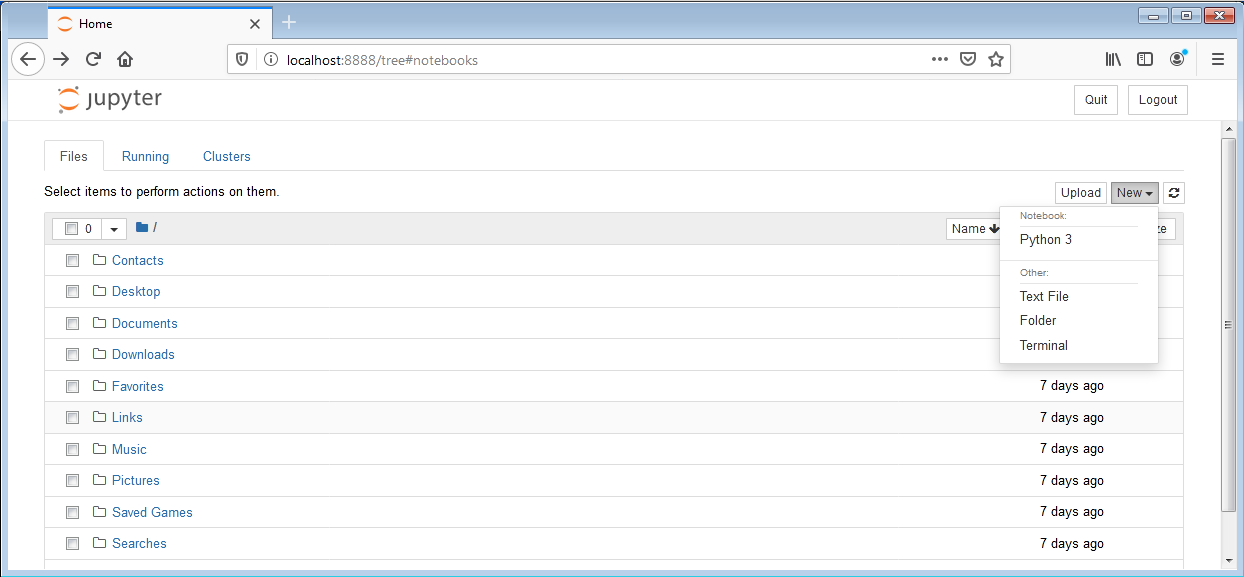
\includegraphics[scale=.5]{pics/jupyter2.png}
    \caption{Aplikasi \texttt{Jupyter}}
    \label{fig:jupyter}
  \end{center}
\end{figure}

\begin{figure}
  \begin{center}
    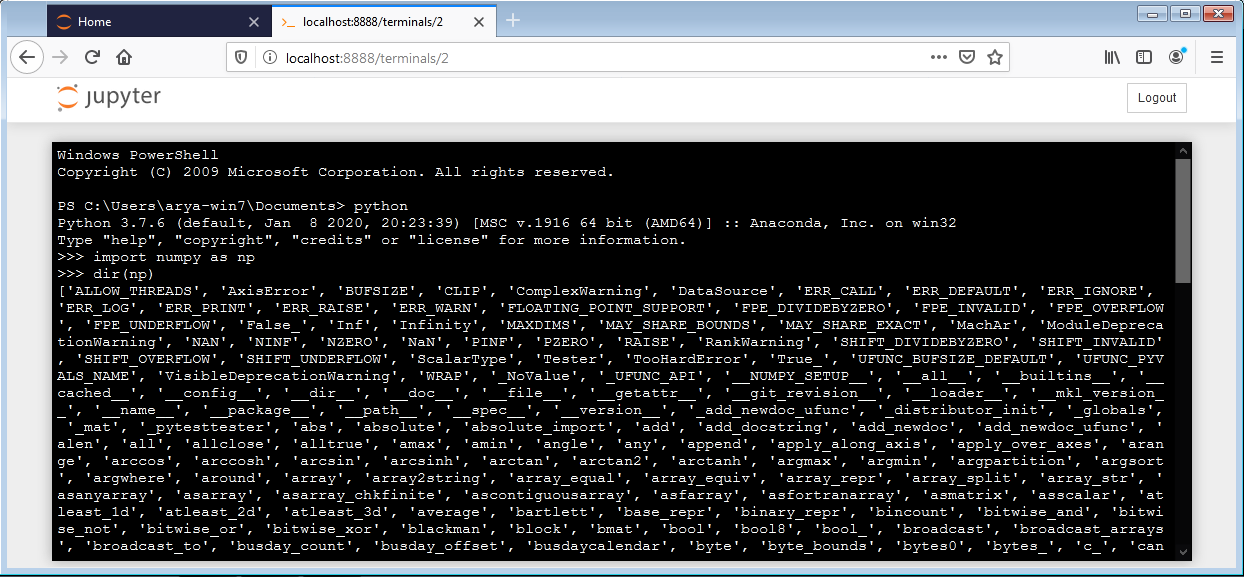
\includegraphics[scale=.5]{pics/jupyter3.png}
    \caption{Terminal pada aplikasi \texttt{Jupyter}}
    \label{fig:jupyterTerminal}
  \end{center}
\end{figure}

\begin{figure}
  \begin{center}
    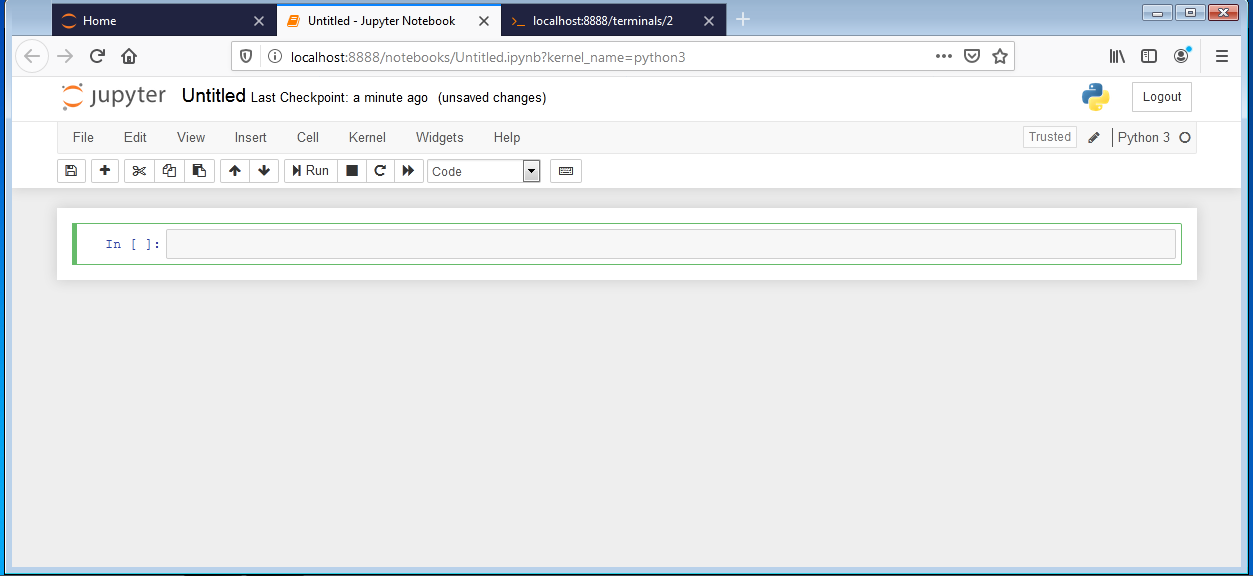
\includegraphics[scale=.5]{pics/jupyter4.png}
    \caption{Python \texttt{Shell} pada aplikasi \texttt{Jupyter}}
    \label{fig:jupyterShell}
  \end{center}
\end{figure}

\begin{figure}[h!]
  \begin{center}
    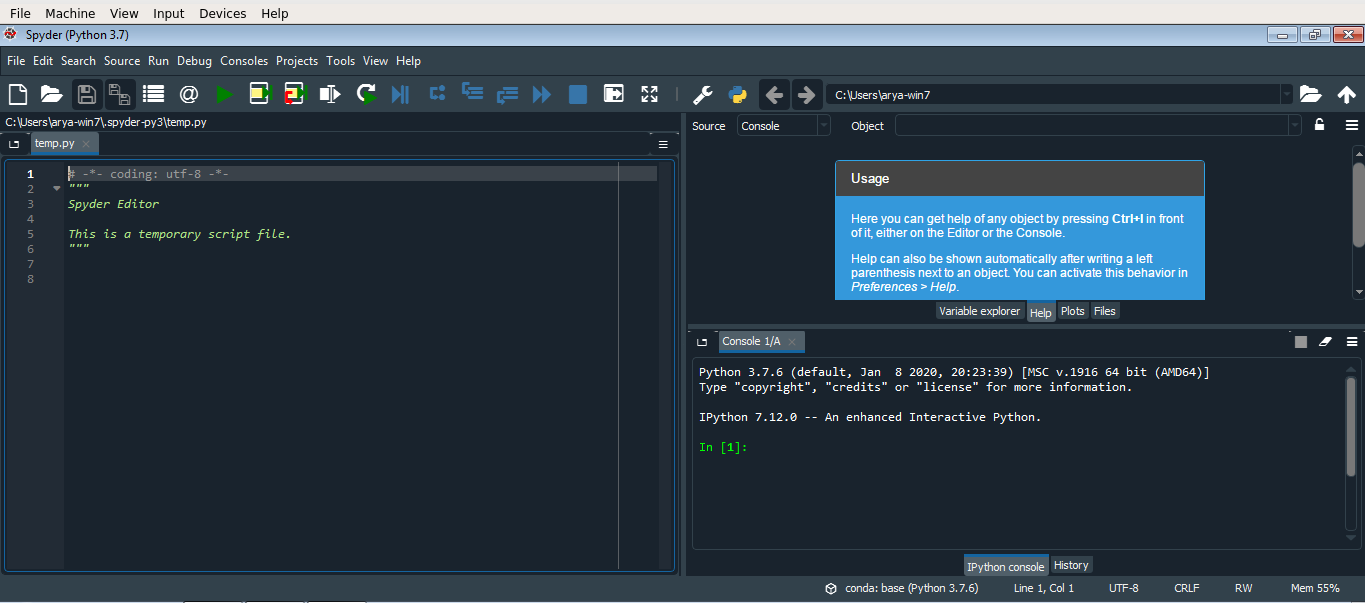
\includegraphics[scale=.45]{pics/spyder.png}
    \caption{Aplikasi \texttt{Spyder}}
    \label{fig:spyder}
  \end{center}
\end{figure}


\chapter{Dasar Pemrograman Python}
\section{Pendahuluan}
Bahasa pemrograman Python memiliki 4 sifat dasar berikut\footnote{\url{https://www.tutorialspoint.com/python/index.htm}}.
\begin{enumerate}
  \item \textit{Interpreter}. Python diproses oleh \textit{interpreter}, sehingga tidak perlu dikompilasi untuk menjalankannya. Hal ini seperti dijumpai pada bahasa pemrograman PHP yang sangat populer itu.
  \item Interaktif. Anda dapat berinteraksi denga Python dengan memberikannya perintah satu per satu melalui Python \texttt{shell}. Setiap perintah yang diberikan langsung akan direspon. Selain itu, Python bersifat \textit{self explained}. Jika ada fungsi dari suatu obyek yang tidak kita ketahui, kita bisa mempelajarinya langsung dari dokumentasi di Python \texttt{shell}.
  \item Berorientasi obyek. Ada semacam slogan bahwa '''\textit{Everything is object in Python}'''. Seperti telah dipahami melalu kuliah Rekayasa Perangkat Lunak, orientasi obyek menyebabkan variabel dan fungsi (sering disebut sebagai \textit{state} dan \textit{behavior}) terkemas dalam sebuah obyek, sehingga memudahkan pengelolaan variabel. Fungsi yang melekat pada sebuah obyek juga dapat diturunkan dari satu obyek ke obyek lain sehingga tidak perlu dideklarasi ulang. Namun, fitur orientasi obyek ini pemberlakuannya bagi pemrogram tidak seketat seperti yang dilakukan di \texttt{Java}. Jika \texttt{Java} mengharuskan pemrogram mendeklarasikan kelas untuk membuat program yang bahkan sangat sederhana, makan Python tidak mengharuskannya.
  \item Bahasa pemrograman untuk pemula. Hal ini disebabkan karena Python sangat sederhana, tidak memerlukan banyak deklarasi yang seringkali menyulitkan, bahkan menakutkan bagi pemula. Selain itu, Python juga mendukung pengembangan aplikasi untuk banyak \textit{platform}, dari aplikasi \textit{embedded} hingga \textit{web} dan \textit{mobile}. 
\end{enumerate}

Untuk sifat dasar pertama dan kedua, dapat dilihat ilustrasinya di \figurename~\ref{fig:interpreter}. Dalam \figurename~\ref{fig:interpreter}, Python \texttt{shell} dipanggil dengan perintah \texttt{python3}. Hal tersebut disebabkan karena Ubuntu (yang sedang digunakan adalah Ubuntu 18.04) secara \textit{default} menyertakan Python versi 2.x. Sedangkan untuk Python versi 3.x harus dijalankan dengan perintah \texttt{python3}. Di \figurename~\ref{fig:interpreter} terlihat bahwa ada dua perintah yang diberikan secara berurutan. Tetapi, Python akan meresponnya satu per satu. Sedangkan untuk keluar dari Python \texttt{shell}, berikan perintah \texttt{exit()}.

\begin{figure}[h!]
  \begin{center}
    \includegraphics[scale=.5]{pics/interpreter.png}
    \caption{Python \texttt{shell} sedang menerima perintah}
    \label{fig:interpreter}
  \end{center}
\end{figure}

Untuk sifat dasar ketiga dapat diilustrasikan melalui \figurename~\ref{fig:obyek}. Kita dapat mengetahui jenis obyek dari variabel \texttt{a} dengan fungsi \texttt{type(a)}. Sedangkan untuk melihat fungsi dan variabel apa saja yang terkandung pada variabel \texttt{a}, kita dapat menggunakan fungsi \texttt{dir(a)}. Tetapi, meskipun semuanya di dalam Python adalah obyek, penggunaan Python tidak mengharuskan kita mendeklarasi kelas secara eksplisit. Dengan menuliskan perintah \texttt{a=3}, Python tahu bahwa obyek \texttt{a} adalah obyek dari kelas \texttt{integer}. Bahkan, di \figurename~\ref{fig:interpreter}, operasi aritmatika dapat dilakukan tanpa mendeklrasi variabel.

\begin{figure}[h!]
  \begin{center}
    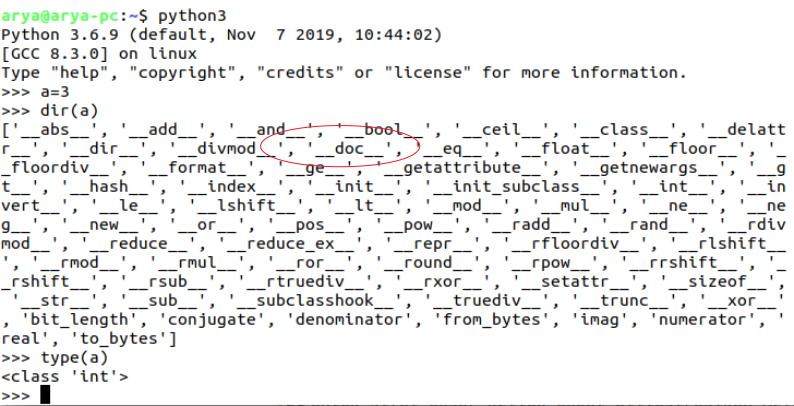
\includegraphics[scale=.5]{pics/interpreter2a.png}
    \caption{Variabel \texttt{a} sebagai obyek}
    \label{fig:obyek}
  \end{center}
\end{figure}

Di \figurename~\ref{fig:obyek} terlihat ada entitas yang diawali dan/atau diakhir dengan karakter dua \textit{underscore} ('\_\_') atau sering disebut sebagi \textit{dunder}\footnote{\url{https://dbader.org/blog/meaning-of-underscores-in-python}} (\textit{double undescore}) oleh komunitas pemrogram Python. Hal tersebut merupakan bagian dari PEP (\textit{Python Enhancement Proposals}) ke-8 tentang \textit{Style Guide for Python Code}\footnote{\url{https://www.python.org/dev/peps/pep-0008/}}.

Di \figurename~\ref{fig:obyek} juga terlihat bahwa obyek \texttt{a} memiliki fungsi \texttt{\_\_doc\_\_}. Fungsi inilah yang akan memberikan penjelasan singkat kepada kita tentang obyek yang sedang menjadi perhatian. Untuk menggunakannya, jalankan perintah \texttt{a.\_\_doc\_\_} seperti ditunjukkan \figurename~\ref{fig:doc}. Dengan \texttt{a} adalah nama variabel untuk obyek yang sedang menjadi perhatian.

\begin{figure}[h!]
  \begin{center}
    \includegraphics[scale=.5]{pics/interpreter3.png}
    \caption{Menampilkan dokumentasi obyek \texttt{integer a}}
    \label{fig:doc}
  \end{center}
\end{figure}

Format dokumentasi seperti yang ditunjukkan pada \figurename~\ref{fig:doc} sulit untuk dipahami. Pendekatan lain untuk mempelajari dokumentasi sebuah pustaka adalah dengan menggunakan fungsi \texttt{help}. Untuk kasus seperti \figurename~\ref{fig:doc}, perintah yang dijalankan adalah \texttt{help(a)} (\textbf{BUKAN} \texttt{a.\_\_doc\_\_}). Hasilnya ditunjukkan pada \figurename~\ref{fig:doc2}. Untuk keluar dari modus dokumentasi tersebut, pengguna tinggal memberi perintah \texttt{q} setelah tanda titik dua (\figurename~\ref{fig:doc2}). Sedangkan untuk melihat isi dokumentasi selanjutnya pengguna dapat menggunkana tombol spasi di papan ketik.

\begin{figure}
  \begin{center}
    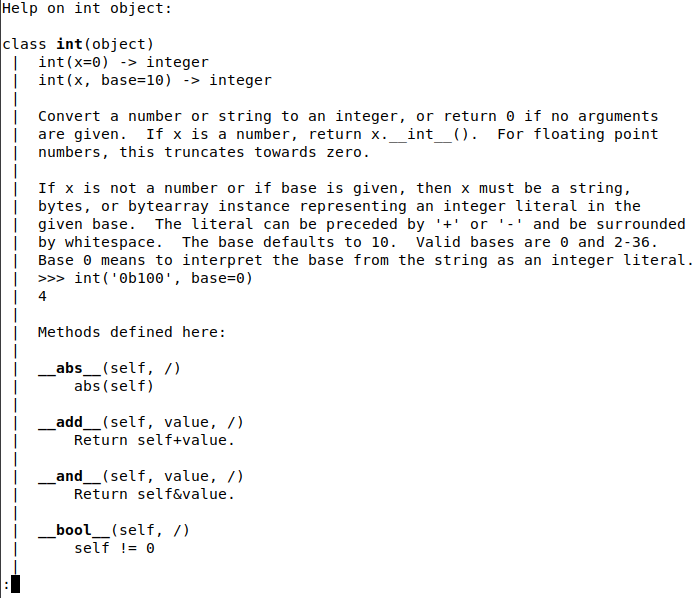
\includegraphics[scale=.5]{pics/interpreter4.png}
    \caption{Menampilkan dokumentasi obyek \texttt{integer a} menggunakan fungsi \texttt{help}}
    \label{fig:doc2}
  \end{center}
\end{figure}

\section{Struktur Data}
%http://thomas-cokelaer.info/tutorials/python/data_structures.html
Strukur data yang dimaksud di sini adalah data \textit{array}/larik dan sejenisnya, serta cara penggunaannya. Tidak jarang, fungsi dalam pustaka \textit{scikit-image} menerima argumen atau mengembalikan nilai dalam bentuk data \textit{array} atau sejenisnya. 
\subsection{\texttt{List}}
\textit{List} adalah \textit{array} yang paling banyak digunakan. Kita dapat menyimpan sejumlah nilai, dari tipe apapun ke dalam \texttt{list}, bahkan menambah atau mengurangi isinya. Untuk yang pernah mempelajari bahasa pemrograman C, tentu paham betapa sulitnya melakukan hal tersebut di C. Untuk C++ \texttt{list} dapat terapkan lebih mudah dengan bantuan \textit{standard template library}\footnote{\url{https://en.wikipedia.org/wiki/Standard\_Template\_Library}}

Sebuah variabel \texttt{list}, misalnya \texttt{a}, diinisiasi dengan perintah \texttt{a=[]}. Maka, variabel \texttt{a} memiliki sejumlah fungsi yang bisa dilihat dengan perintah \texttt{dir(a)}. Diktat ini hanya akan membahas fungsi-fungsi yang sering digunakan saja. Fungsi lain bisa dipelajari sendiri dengan bantuan perintah \texttt{help(a.nama\_fungsi)}, dengan \texttt{a} adalah obyek \texttt{list}.

\begin{enumerate}
  \item \texttt{append}. Fungsi ini menambahkan elemen baru ke variabel \texttt{list}. Perhatikan \figurename~\ref{fig:append}. Variabel \texttt{a} yang awalnya kosong, kemudian diisi satu per satu menggunakan perintah \texttt{append}. Variabel \texttt{a} terakhir memiliki dua elemen, masing-masing bertipe \texttt{integer} dan \texttt{character}.
  \begin{figure}
    \begin{center}
      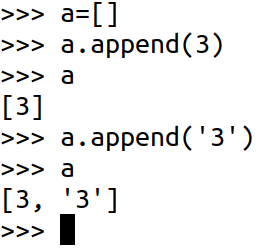
\includegraphics[scale=1.25]{pics/append.png}
      \caption{Proses penambahan elemen \texttt{list}}
      \label{fig:append}
    \end{center}
  \end{figure}
  
  \item \texttt{extend}. Fungsi ini memiliki tugas yang sama dengan \texttt{append} dengan sedikit perbedaan. Perhatikan \figurename~\ref{fig:extend}. Di \figurename~\ref{fig:extend1}, variabel \texttt{a} ditambahkan sebuah elemen berupa variabel list \texttt{b} menggunakan fungsi \texttt{append}. Variabel \texttt{b} yang telah memiliki dua elemen ditambahkan ke variabel \texttt{a} sebagai satu elemen. Hal tersebut terlihat dari dijalankannya perintah \texttt{len(a)}.
  
Sementara di \figurename~\ref{fig:extend2}, proses yang sama dilakukan menggunakan fungsi \texttt{extend}. Fungsi \texttt{extend} akan menambahkan variabel \texttt{b} ke dalam variabel \texttt{a} tidak sebagai \texttt{list} secara keseluruhan, tetapi menambahkan masing-masing elemen variabel \texttt{b} ke dalam \texttt{a}. Itu sebabnya, hasil penambahan \texttt{b} ke dalam \texttt{a} membuat \texttt{a} saat ini memiliki dua elemen.
  
\begin{figure}[h!]
\begin{center}
\subfigure[]{\label{fig:extend1}}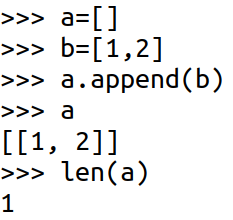
\includegraphics[scale=1.25]{pics/extend1.png}
\subfigure[]{\label{fig:extend2}}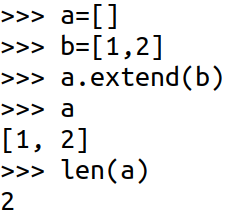
\includegraphics[scale=1.25]{pics/extend2.png}
\caption{Perbandingan penambahan elemen \texttt{list} menggunakan fungsi (a). \texttt{append} dan (b). \texttt{extend}}
\label{fig:extend}
\end{center}
\end{figure}
Di \lstlistingname~\ref{lst:pynonxmlreader}, ditunjukkan variabel \texttt{list} yang salah satunya digunakan sebagai kriteria \textit{looping}, tepatnya dilakukan oleh variabel \texttt{hilang} yang dideklarasikan di baris ke-9.

\item \texttt{insert}. Selain menambahkan elemen ke variabel \texttt{list} di posisi akhir, penambahan elemen juga dapat dilakukan di posisi tertentu. Perhatikan \figurename~\ref{fig:insert}. Penambahan karakter \texttt{'x'} pada posisi pertama dari \texttt{list} dilakukan dengan perintah \texttt{a.insert(0,'x')}. Hal ini disebabkan karena indeks dari elemen \texttt{list} dimulai dari \texttt{0}. 

\begin{figure}[h!]
  \begin{center}
    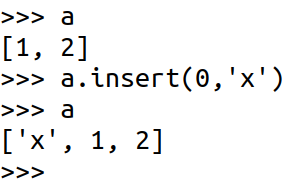
\includegraphics[scale=1.25]{pics/insert.png}
    \caption{Penambahan karakter 'x' ke variabel \texttt{a} di posisi pertama}
    \label{fig:insert}
  \end{center}
\end{figure}

\item \texttt{remove}. Selain menambahkan elemen ke variabel \texttt{list}, kita dapat juga membuang salah satu elemen yang ada di posisi tertentu di dalam \texttt{list}. Perhatikan figurename~\ref{fig:remove}. Perintah \texttt{remove} digunakan untuk mengeluarkan elemen tertentu dari \texttt{list}. Jika ada lebih dari satu elemen yang sama yang akan dikeluarkan, maka elemen terpilih untuk dikeluarkan adalah elemen yang muncul pertama kali pada \texttt{list}.

\begin{figure}[h!]
  \begin{center}
    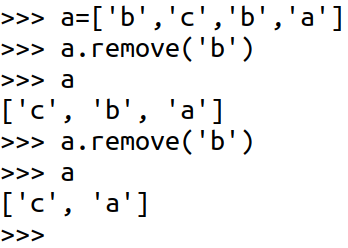
\includegraphics[scale=1.25]{pics/remove.png}
    \caption{Mengeluarkan elemen tertentu dari \texttt{list}}
    \label{fig:remove}
  \end{center}
\end{figure}

\item \texttt{pop}. Fungsi ini akan mengeluarkan elemen terakhir dari \texttt{list}. Perhatikan \figurename~\ref{fig:pop}.

\begin{figure}[h!]
  \begin{center}
    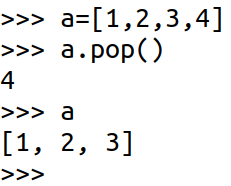
\includegraphics[scale=1.25]{pics/pop.png}
    \caption{Mengeluarkan elemen terakhir dari variabel \texttt{list}}
    \label{fig:pop}
  \end{center}
\end{figure}

\end{enumerate}
\subsection{\texttt{Tuple}}
\texttt{Tuple} adalah jenis \textit{array} selain \texttt{list} yang di Python dideklarasikan dengan perintah \texttt{a=()}. Operasi pada \texttt{tuple} lebih cepat dilakukan jika dibandingkan dengan \texttt{list}. Hal ini disebabkan karena \texttt{tuple} bersifat statis karena elemen yang ada di dalamnya tidak dapat diubah, kecuali yang bersifat \textit{mutable}. Karena bersifat statis, deklarasi variabel \texttt{a=()} tidak akan bermanfaat. Perhatikan \figurename~\ref{fig:tuple}.

Di \figurename~\ref{fig:tuple}, sebuah variabel \texttt{a} memiliki empat elemen, di mana elemen ke-4 merupakan sebuah \texttt{list}. Elemen ke-4 diakses dengan indeks \texttt{3} (karena indeks \texttt{tuple} dimulai dari \texttt{0}). Ketika diakes, isi dari elemen ke-4 tersebut dapat diubah karena bersifat \textit{mutable}. Sebaliknya, ketika elemen lain (dalam hal ini elemen ke-2) akan diubah nilainya, Python menolaknya. 

\begin{figure}[h!]
  \begin{center}
    \includegraphics{pics/tuple.png}
    \caption{Beberapa operasi yang dilakukan pada variabel \texttt{tuple}}
    \label{fig:tuple}
  \end{center}
\end{figure}

Untuk \lstlistingname~\ref{lst:pynonxmlreader}, variabel \texttt{hilang} yang dideklarasikan di baris ke-9 sebagai variabel \texttt{list}, dapat juga dideklarasikan sebagai \texttt{tuple}. Hal ini disebabkan karena sepanjang \lstlistingname~\ref{lst:pynonxmlreader} dijalankan, elemen yang tersimpan di dalam variabel \texttt{hilang} tidak berubah. 
 
\subsection{\texttt{Dictionary}}
\texttt{Dictionary} merupakan \textit{array} yang elemen penyusunnya merupakan pasangan \textit{key-value}. Setiap elemen akan diindeks berdasarkan \textit{key}. \texttt{Dictionary} dideklarasikan menggunakan perintah \texttt{a=\{\}}. Untuk menambah elemen ke variabel \texttt{dictionary}, gunakan perintah seperti \figurename~\ref{fig:dict}.

\begin{figure}[h!]
  \begin{center}
    \includegraphics[scale=1.25]{pics/dictionary.png}
    \caption{Menambahkan elemen ke variabel \texttt{dictionary}}
    \label{fig:dict}
  \end{center}
\end{figure}

Kita juga dapat mengeluarkan sebuah elemen dari variabel \texttt{dictionary}. Karena elemennya merupakan pasangan \textit{key-value}, maka ketika dikeluarkan, pasangan \textit{key-value} tersebut tidak ada lagi di variabel \texttt{dictionary}. Perhatikan \figurename~\ref{fig:popDict}, elemen yang memiliki \textit{key} berupa karakter \texttt{'nama'} akan dikeluarkan menggunakan fungsi \texttt{pop}. Karena memerlukan argumen berupa \textit{key}, maka fungsi \texttt{pop} dapat mengeluarkan elemen yang posisinya di mana saja di dalam variabel \texttt{dictionary}, tidak harus di posisi terakhir.  

\begin{figure}[h!]
  \begin{center}
    \includegraphics[scale=1.25]{pics/popDict.png}
    \caption{Mengeluarkan pasangan \textit{key-value} dari variabel \texttt{dictionary}}
    \label{fig:popDict}
  \end{center}
\end{figure}

\section{Operasi Berkas}

Yang dimaksud sebagai operasi berkas di sub bab ini ditujukan untuk memberikan solusi otomatis melakukan operasi pengolahan citra pada sejumlah besar citra (khususny), atau berkas digital secara umum. Sebagai ilustrasi, dataset citra terkait tumbuhan salah satunya dapat diperoleh di PlantCLEF2017 \footnote{\url{http://otmedia.lirmm.fr/LifeCLEF/PlantCLEF2017/TrainPackages/PlantCLEF2017Train1EOL.tar.gz}}.

Ketika berkas tersebut diekstrak, kita akan memperoleh \texttt{directory} data sebagai \texttt{directory} teratas dari dataset. Di dalamnya ada cukup banyak \texttt{directory} yang diberi nama berupa deretan angka. Di dalam \texttt{directory} tersebut, akan ada pasangan berkas dengan nama sama dari jenis \texttt{xml} dan \texttt{jpg}. Isi dari berkas berekstensi \texttt{xml} ditunjukkan oleh \lstlistingname~\ref{lst:135788}. Berkas ini berada dalam \texttt{directory} \texttt{9982}.

\scriptsize
\lstinputlisting[language=xml, numbers=left, numberstyle=\tiny, caption=135788.xml, showstringspaces=false, label=lst:135788]{script/135788.xml}
\normalsize

Yang perlu diperhatikan dari \texttt{element} berkas \texttt{xml} di \lstlistingname~\ref{lst:135788} adalah sebagai berikut.
\begin{itemize}
  \item \texttt{FileName}: elemen ini berisi informasi nama berkas
  \item \texttt{Content}: elemen ini berisi informasi jenis citra. \lstlistingname~\ref{lst:135788} menunjukkan bahwa citra yang sedang diamati adalah bunga.
  \item \texttt{Family}, \texttt{Genus}, \texttt{Species}: masing-masing menunjukkan tingkatan taksonomi dari tumbuhan. Dalam konteks klasifikasi tanaman, umumnya informasi spesies yang diperlukan. Tetapi, karena berkas pada dataset tidak tersusun dalam taksonomi, maka informasi yang disimpan pada elemen tersebut bermanfaat ketika kita ingin menyusun ulang struktur berkas citra berdasarkan taksonominya.
\end{itemize}

Operasi berkas yang dicontohkan dalam diktat ini adalah menyusun ulang citra berdasarkan jenis citra, apakah itu bunga atau daun. Kemudian di dalam \textit{directory} jenis citra tersebut, citra akan disusun mengikuti hirarki taksonominya. Sehingga akan ada struktur \textit{directory} seperti \texttt{Flower/Compositae/Carthamus/Carthamus\ caeruleus\ L.}. Pada kasus ini, berkas-berkas di dalamnya merupakan bunga dari \texttt{Family Compositae}, \texttt{Genus Carthamus} dan \texttt{Species Carthamus\ caeruleus\ L.}. Programnya disajikan pada \lstlistingname~\ref{lst:pynonxmlreader}. Di dalamnya ada sejumlah operasi berkas seperti pencarian dalam \textit{directory} tertentu, pencarian berkas dengan ekstensi tertentu sampai membuat \textit{directory} dan menduplikasi berkas dari satu \textit{directory} ke \textit{directory} lain.

\scriptsize
\lstinputlisting[language=python, numbers=left, numberstyle=\tiny, caption=Menysun ulang struktur berkas, showstringspaces=false, label=lst:pynonxmlreader]{script/pynonxmlreader.py}
\normalsize

Di \lstlistingname~\ref{lst:pynonxmlreader} disediakan juga pendeteksi kesalahan \texttt{try-except} ketika operasi berkas dilakukan. Hal ini dimaksudkan agar jalannya program tidak terhenti ketika kesalahan terjadi. Pengguna cukup mengetahui dari pesan kesalahan yang didefinisikan.

Jika fokus penelitian kita hanya pada bunga, maka kita hanya akan melakukan pengolahan pada citra yang berisi obyek bunga. Demikian juga untuk \texttt{Family}, \texttt{Genus} maupun \texttt{Species} tertentu.

Pada kondisi tertentu, misalnya seperti ditunjukkan \lstlistingname~\ref{lst:301518}, tidak ada informasi jenis citra. Hal ini terlihat dari tidak adanya isi elemen \texttt{Content}. Untuk citra yang salah satu atau seluruh elemennya tidak bernilai, \lstlistingname~\ref{lst:pynonxmlreader} akan mengelompokkannya sebagai \texttt{Undefined}. Untuk citra yang dideskripsikan oleh berkas \texttt{xml} seperti \lstlistingname~\ref{lst:301518} akan disimpan dalam \textit{directory} \texttt{Undefined/Pinaceae/Pinus/Pinus\ pinea\ L.}.

\scriptsize
\lstinputlisting[language=xml, numbers=left, numberstyle=\tiny, caption=Contoh citra tanpa informasi jenis, showstringspaces=false, label=lst:301518]{script/301518.xml}
\normalsize

Operasi pencarian semua berkas pada \textit{directory} tertentu juga bermanfaat ketika diperlukan operasi pengolahan citra seperti \texttt{resize} atau \texttt{rescale}. Fitur \textit{Histogram of Oriented Gradients} seperti akan dijelaskan pada sub bab \ref{sec:hog} sangat dipengaruhi oleh ukuran citra. Sehingga citra yang akan dianalisis harus dalam ukuran yang sama untuk mengetahui aspek pembedanya, yaitu obyek yang terdapat di dalam citra. Tentu tidak efisien jika operasi \texttt{resize} atau \texttt{rescale} harus dilakukan secara manual.


\chapter{Pendahuluan Pustaka \texttt{Scikit-Image}}

\chapter{Sub Modul Pustaka \texttt{Scikit-Image}}

\bibliographystyle{apalike}
\bibliography{reference}
\end{document}
